\chapter{Prototipação}

Neste capítulo será abordado o processo de desenvolvimento do protótipo da solução, mostrando as soluções tomadas e descrições das telas do aplicativo, assim como suas funcionalidades.

\section{Escolha da ferramenta para prototipação}

O processo para desenvolvimento do protótipo interativo foi iniciado após as definições da arquitetura e desenho dos diagramas citados anteriormente. No início foram feitas pesquisas e análises das melhores ferramentas para prototipagem. Os critérios iniciais buscados para a ferramenta de prototipagem foram: interface amigável, funcionalidades que possibilitem criar um protótipo interativo, compartilhamento de projeto em nuvem, liberdade na criação de \textit{layouts} e customização de componentes de tela, além de não ter custo em sua utilização.

Foram identificadas duas ferramentas que atendem esses requisitos, sendo \textit{Adobe XD} e \textit{Figma}. Foi iniciado o desenvolvimento do protótipo no \textit{Adobe XD}. O \textit{Adobe XD} atendeu a expectativa para a criação das telas interativas do protótipo, contudo, após uma nova avaliação, foi visto que o \textit{Figma} possui a possibilidade de duas ou mais pessoas atuarem de forma síncrona no mesmo projeto através do navegador, possibilitando uma maior agilidade para os autores deste trabalho prosseguirem com o desenvolvimento do protótipo.

Deste modo, foi feita a migração do projeto do \textit{Adobe XD} para o \textit{Figma}, o que não apresentou problemas visto que o \textit{Figma} tem compatibilidade com arquivos com a extensão do \textit{Adobe XD}. A partir desse ponto foi continuado o desenvolvimento do protótipo, com reuniões para revisão e aplicação de melhorias necessárias, além de realização de \textit{backup} do projeto para controle de versão. Na Figura \ref{fig:figma} é apresentado a interface gráfica do \textit{Figma}.

\begin{figure}[H]
    \centering
    \caption{Interface do Figma}
    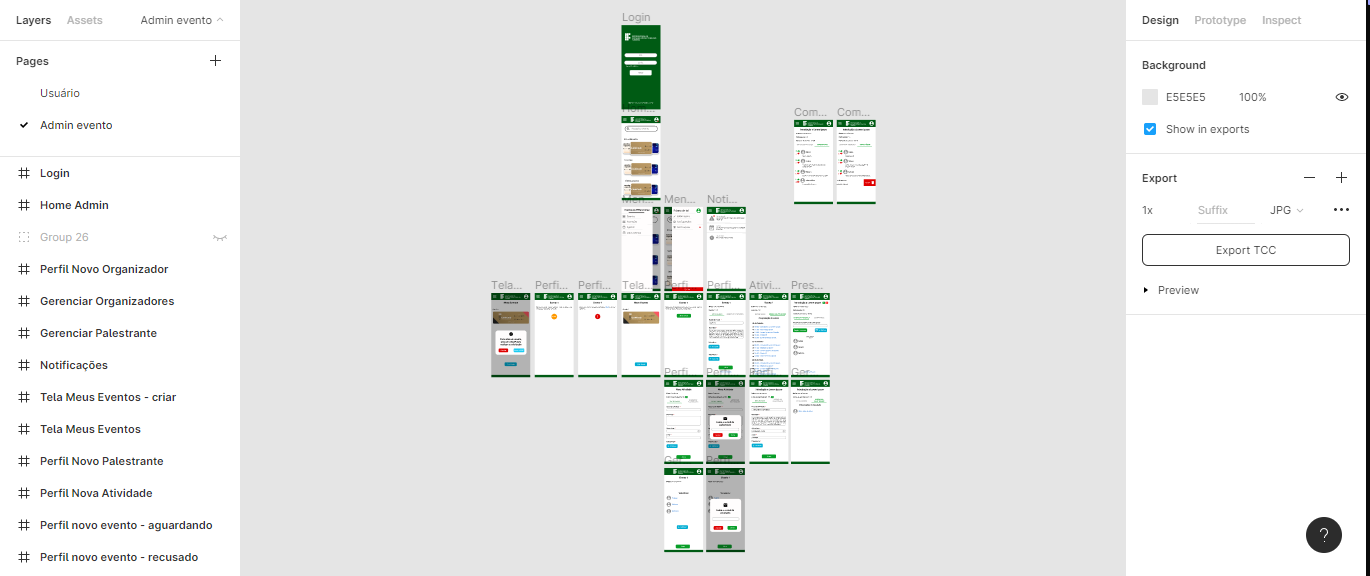
\includegraphics[scale=0.44]{figuras/figma.PNG}
    \label{fig:figma}
    \legend{Fonte: \textit{website} do \textit{Figma}}
\end{figure}

\section{Perfis de usuário do aplicativo Eventos IFF}

O aplicativo Eventos IFF possui quatro perfis de usuário relacionados a cada evento, send assim, para cada evento o usuário pode assumir um perfil diferente, dependendo da sua interação com o evento na plataforma. Ao todo são 4 perfis, os quais são listados a seguir:

\begin{itemize}
    \item Audiência: usuário que realiza a inscrição no evento, atuando como participante do mesmo e de suas atividades;
    \item Organizador: é o criador do evento. Esse usuário pode realizar todas as ações relacionadas a gestão de evento no aplicativo;
    \item Voluntário: é o usuário convidado pelo o organizador para atuar na gestão do evento através do aplicativo, no entanto com limitação de ações;
    \item Palestrante: também é um usuário convidado pelo organizador para atuar na gestão do evento, porém ele tem relação apenas com a(s) atividade(s) a qual ele foi convidado para atuar, limitando-se apenas a realizar ações nessa(s) atividade(s).
\end{itemize}

Cada perfil possui as funcionalidades que podem ser executadas no determinado evento, baseando-se em suas respectivas responsabilidades no respectivo evento. Na Tabela \ref{tab:funcionalidades} é relacionado as funcionalidades do aplicativo com os perfis de usuários.

\begin{table}[]
\caption{Relação das funcionalidades e perfis do aplicativo Eventos IFF}
\label{tab:funcionalidades}
\begin{tabular}{|l|l|c|l|l|}
\hline
 & \multicolumn{1}{c|}{Palestrante} & Organizador & \multicolumn{1}{c|}{Voluntário} & \multicolumn{1}{c|}{Audiência} \\ \hline
Registrar presença & \multicolumn{1}{c|}{x} & x & \multicolumn{1}{c|}{x} &  \\ \hline
Criar atividade &  & x &  &  \\ \hline
Editar atividade &  & x & \multicolumn{1}{c|}{x} &  \\ \hline
Excluir atividade &  & x &  &  \\ \hline
Ativar evento &  & x &  &  \\ \hline
Editar evento &  & x &  &  \\ \hline
Convidar usuário para gestão &  & x &  &  \\ \hline
Criar comentário &  & \multicolumn{1}{l|}{} &  & \multicolumn{1}{c|}{x} \\ \hline
Denunciar comentário &  & \multicolumn{1}{l|}{} &  & \multicolumn{1}{c|}{x} \\ \hline
Avaliar comentário &  & \multicolumn{1}{l|}{} &  & \multicolumn{1}{c|}{x} \\ \hline
Excluir comentário & \multicolumn{1}{c|}{x} & x & \multicolumn{1}{c|}{x} & \multicolumn{1}{c|}{x} \\ \hline
Inscrever em evento &  & \multicolumn{1}{l|}{} &  & \multicolumn{1}{c|}{x} \\ \hline
Solicitar emissão de certificado &  & x &  & \multicolumn{1}{c|}{x} \\ \hline
\end{tabular}
\legend{\newline Fonte: elaborado pelos autores}
\end{table}

\section{Jornada do usuário com perfil audiência}

Ao iniciar o aplicativo é necessário realizar a autenticação através da tela de \textit{login} (Figura \ref{fig:audiencia1}), possibilitando também criar cadastro e alterar senha caso o usuário não se lembre da senha. As ações de cadastro e redefinição de senha redirecionam o usuário para o \textit{website} Eventos IFF.

\begin{figure}[H]
    \centering
    \caption{Tela de \textit{login}}
    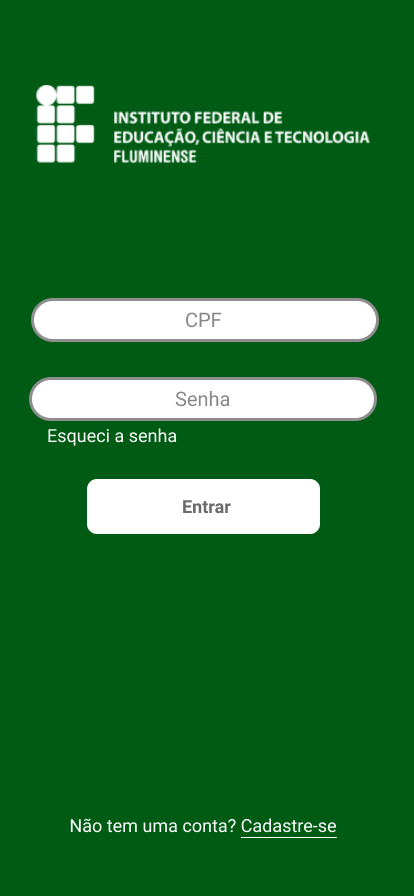
\includegraphics[scale=0.44]{figuras/Audiencia/1-Login.jpg}
    \label{fig:audiencia1}
    \legend{Fonte: elaborado pelos autores}
\end{figure}

Após a autenticação, é aberto como tela inicial a exibição dos eventos em cartões contendo as imagens de capa do evento, dispostas com efeito carrossel, dividindo os eventos em andamento, eventos classificados como favoritos pelo usuário e eventos já finalizados (Figura \ref{fig:audiencia2}). Além disso, há um campo textual localizado no topo da tela que possibilita o usuário a buscar o evento desejado pelo nome.

\begin{figure}[H]
    \centering
    \caption{Tela inicial}
    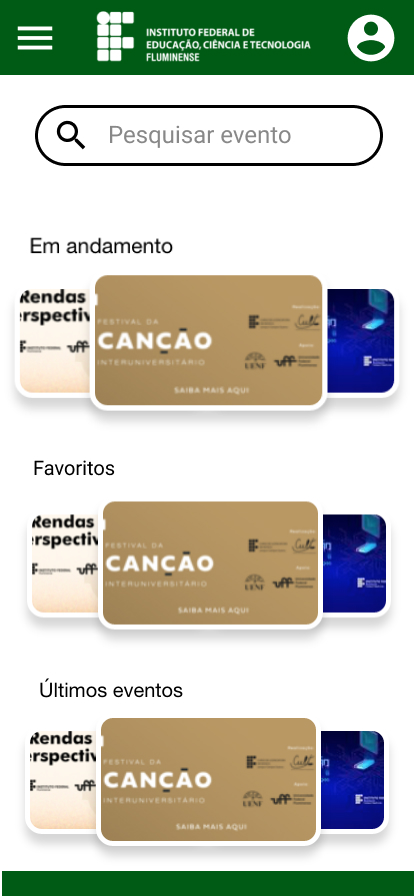
\includegraphics[scale=0.44]{figuras/Audiencia/2-TelaPrincipal.jpg}
    \label{fig:audiencia2}
    \legend{Fonte: elaborado pelos autores}
\end{figure}

Ao lado esquerdo da tela inicial, no canto superior, há um ícone relacionado ao menu lateral de navegação, acessando o mesmo será feita a abertura do menu lateral (Figura \ref{fig:audiencia3}), onde possui três opções: eventos, inscrições e agenda. Essas opções tem como respectivas ações:

\begin{itemize}
    \item Eventos: redireciona o usuário para a tela inicial do aplicativo, a qual é descrita anteriormente;
    \item Inscrições: abre uma tela, com a mesma estrutura da interface da tela inicial, no entanto apenas os eventos onde o usuário é inscrito é apresentado;
    \item Agenda: apresenta a agenda das atividades dos eventos onde o usuário está inscrito, separados por dia e hora.
\end{itemize}

\begin{figure}[H]
    \centering
    \caption{Menu lateral esquerdo}
    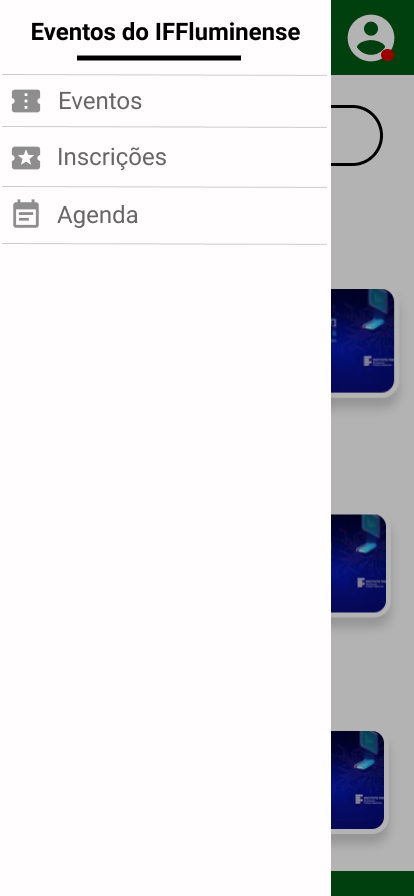
\includegraphics[scale=0.44]{figuras/Audiencia/3-MenuEsquerdo.jpg}
    \label{fig:audiencia3}
    \legend{Fonte: elaborado pelos autores}
\end{figure}

Já ao lado direito, no canto superior da tela, há o ícone exibindo a silhueta de um usuário, a qual sendo selecionada abre o menu lateral de perfil (Figura \ref{fig:audiencia4}.B), que contém opções que possibilitam a edição de dados pessoais, configurações do aplicativo e possíveis notificações direcionadas ao usuário. Essas notificações são relacionadas aos eventos onde o usuário está inscrito (Figura \ref{fig:audiencia4}.A), com isso, quando houver alterações em alguma atividade onde usuário confirmou presença ou faltam 15 minutos para a atividade ser iniciada, uma notificação é enviada para o usuário e listada nessa tela de notificações. Quando houver alguma notificação nova não lida pelo usuário, um círculo vermelho deve ficar ao lado direito da opção "Notificações", como ilustrado na Figura \ref{fig:audiencia4}.B, sendo que após o usuário abrir a tela de notificações, este círculo deve desaparecer.

\begin{figure}[H]
    \centering
    \caption{(A) Tela de notificações. (B) Menu lateral direito.}
    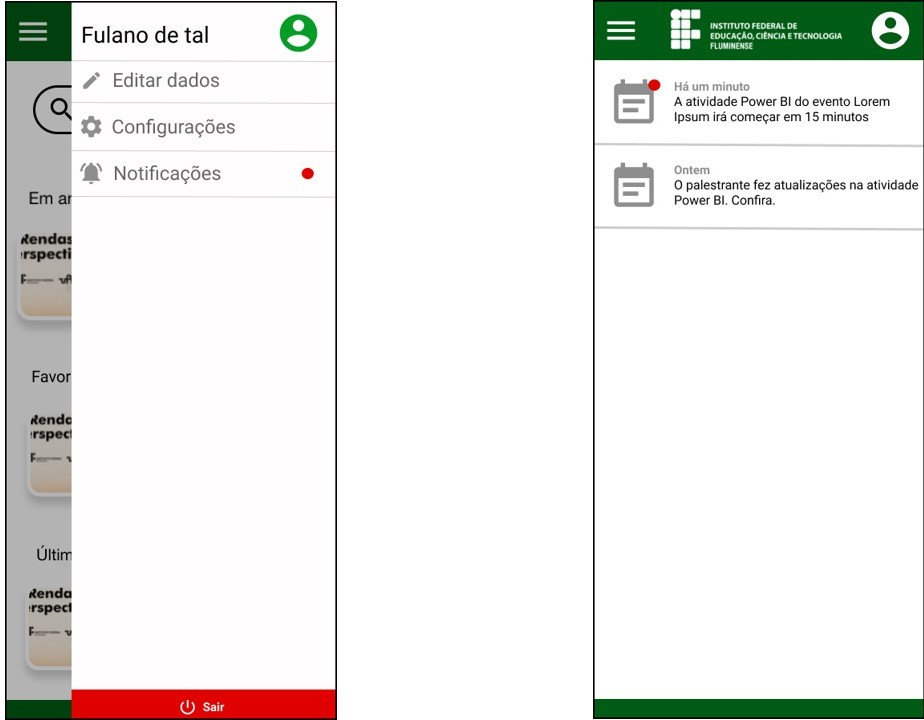
\includegraphics[scale=0.63]{figuras/Audiencia/4-5.jpg}
    \label{fig:audiencia4}
    \legend{Fonte: elaborado pelos autores}
\end{figure}

Para acessar algum evento, o usuário pode selecionar o cartão desejado na tela inicial (Figura \ref{fig:audiencia1}), onde exibirá em uma nova tela os detalhes a respeito do evento (Figura \ref{fig:audiencia6}). Nesta tela está disposta a capa do evento, nome do evento e uma descrição. Se o usuário não estiver inscrito no evento, abaixo da capa estarão disponíveis três botões. Um botão para realizar a inscrição no evento, um botão com um ícone de calendário para abrir as atividades daquele evento, e um botão com um ícone de compartilhamento que permite o usuário compartilhar o evento em outros aplicativos instalados no seu dispositivo móvel.

\begin{figure}[H]
    \centering
    \caption{Tela de inscrição no evento quando o usuário não está inscrito}
    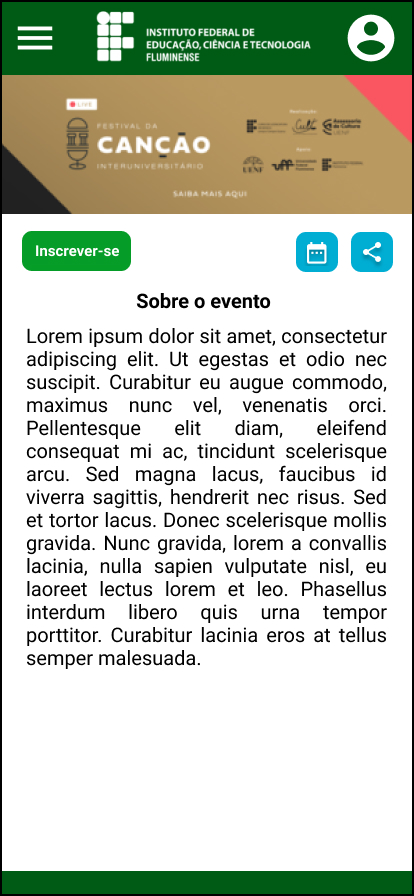
\includegraphics[scale=0.44]{figuras/Audiencia/6-Evento.jpg}
    \label{fig:audiencia6}
    \legend{Fonte: elaborado pelos autores}
\end{figure}

Ao selecionar o botão de inscrição, o status do usuário muda para inscrito no evento, mudando a aparência e texto do botão, indicando que a ação foi realizada com sucesso (Figura \ref{fig:audiencia7}). Além disso, mais dois botões se tornam visíveis abaixo da capa. Um botão com um ícone de \textit{QRCode}, que possibilita ao usuário visualizar o \textit{QRCode} com as credenciais para o mesmo registrar a presença no evento, e outro botão que permite o usuário registrar o evento na lista de eventos favoritos.

\begin{figure}[H]
    \centering
    \caption{Tela de inscrição no evento com a inscrição realizada}
    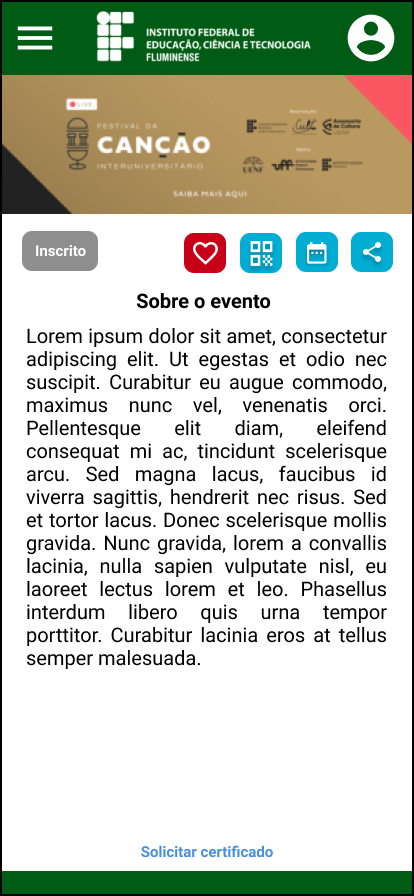
\includegraphics[scale=0.44]{figuras/Audiencia/7-EventoInscrito.jpg}
    \label{fig:audiencia7}
    \legend{Fonte: elaborado pelos autores}
\end{figure}
   
O botão com o ícone de calendário, ao ser acessado, exibe as atividades existentes no evento em uma nova tela (Figura \ref{fig:audiencia8}). As atividades são dispostas em formato lista e divididas por dia, em cada data da lista existe um botão com ícone de calendário, que possibilita assim ao usuário marcar na agenda do dispositivo móvel utilizado as atividades desejadas, tendo como função avisar previamente antes da atividade iniciar.

\begin{figure}[H]
    \centering
    \caption{Tela das atividades do evento}
    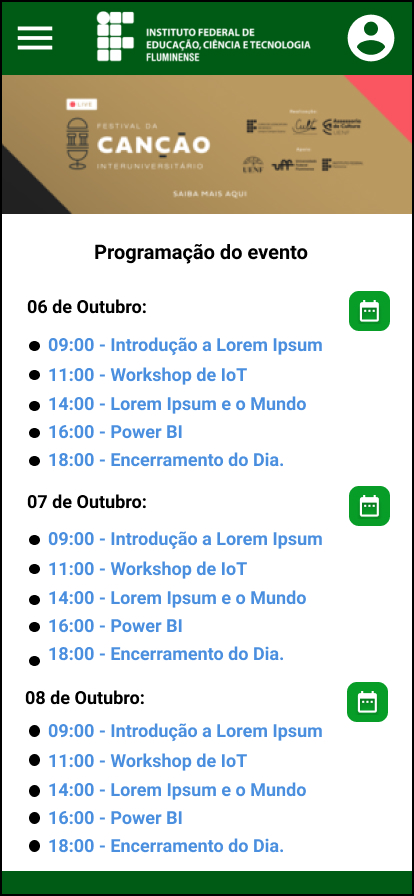
\includegraphics[scale=0.44]{figuras/Audiencia/8-ListaAtividades.jpg}
    \label{fig:audiencia8}
    \legend{Fonte: elaborado pelos autores}
\end{figure}

O usuário poderá acessar a tela da atividade que deseja visualizar selecionando atividade na lista, nessa tela o mesmo poderá efetuar a inscrição na atividade desejada através do botão “Participar” (Figura \ref{fig:audiencia9}). Nesta mesma tela é apresentado informações sobre a respectiva atividade, como nome, data de realização, descrição e endereço ou localização da atividade.

\begin{figure}[H]
    \centering
    \caption{Tela da atividade selecionada}
    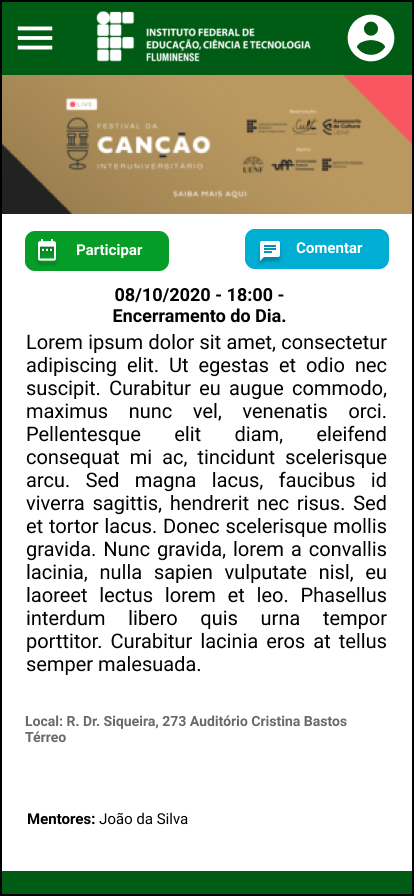
\includegraphics[scale=0.44]{figuras/Audiencia/9-Ativade.jpg}
    \label{fig:audiencia9}
    \legend{Fonte: elaborado pelos autores}
\end{figure}

O usuário pode realizar a ação de enviar um comentário para atividade inscrita, através do botão “Comentar” nesta tela. Após selecionar esse botão, o usuário é redirecionado para a tela de comentários da atividade, onde é exibido os comentários registrados pelos participantes da atividade (Figura \ref{fig:audiencia10}). Cada comentário tem três opções no lado direito, sendo um ícone de avaliação positiva, um ícone avaliação negativa, e um ícone para denunciar o comentário.

\begin{figure}[H]
    \centering
    \caption{Tela de comentários da atividade}
    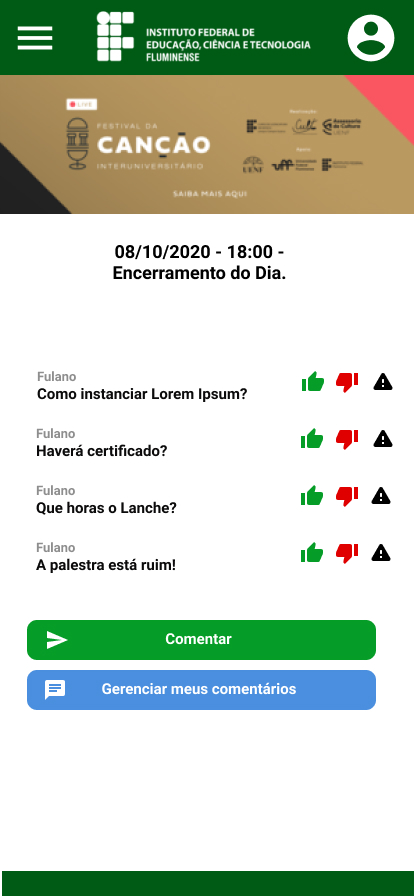
\includegraphics[scale=0.44]{figuras/Audiencia/10-Comentarios.jpg}
    \label{fig:audiencia10}
    \legend{Fonte: elaborado pelos autores}
\end{figure}

Os ícones de avaliação tem o objetivo de ajudar na ordenação da lista de comentários, tendo um aspecto colaborativo entre os participantes da atividade. A avaliação positiva atribui 1 ponto positivo no comentário, e a avaliação negativa atribui 1 ponto negativo. Os comentários são ordenados de forma decrescente pela a diferença desses pontos, sendo o comentário com a maior diferença estando no topo da lista, dando assim maior destaque aos comentários com melhor avaliação.

O ícone para denunciar o comentário emite uma notificação para os usuários organizador, voluntário e palestrante, sendo estes tendo a possibilidade de excluir o comentário. Ao selecionar o ícone para denuncia, o aplicativo deve apresentar uma caixa de dialogo para confirmar a ação, assim como apresentado na Figura \ref{fig:audiencia11}.

\begin{figure}[H]
    \centering
    \caption{Mensagem de confirmação da denuncia de comentário}
    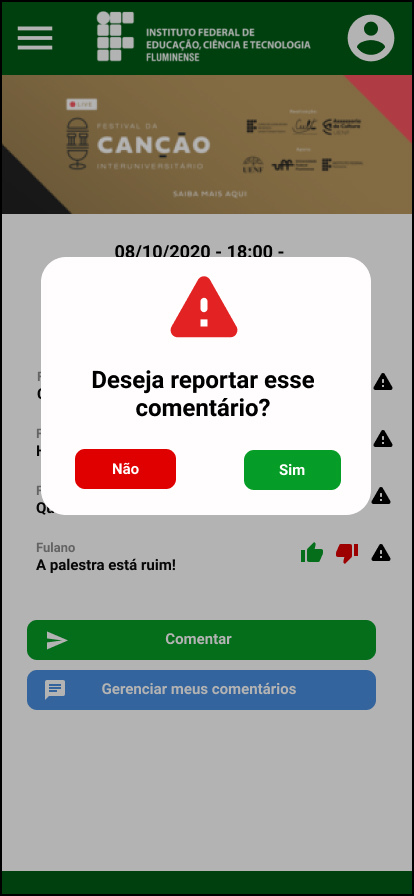
\includegraphics[scale=0.44]{figuras/Audiencia/11-Denunciar.jpg}
    \label{fig:audiencia11}
    \legend{Fonte: elaborado pelos autores}
\end{figure}

Na parte inferior dessa tela há dois botões. O primeiro direciona o usuário para uma tela onde o mesmo pode realizar um comentário novo (Figura \ref{fig:audiencia13}). O segundo botão permite ao usuário visualizar seus comentários realizados naquela atividade, onde o mesmo poderá executar a ação de excluir um ou mais desses comentários.

\begin{figure}[H]
    \centering
    \caption{Tela de envio de um novo comentário}
    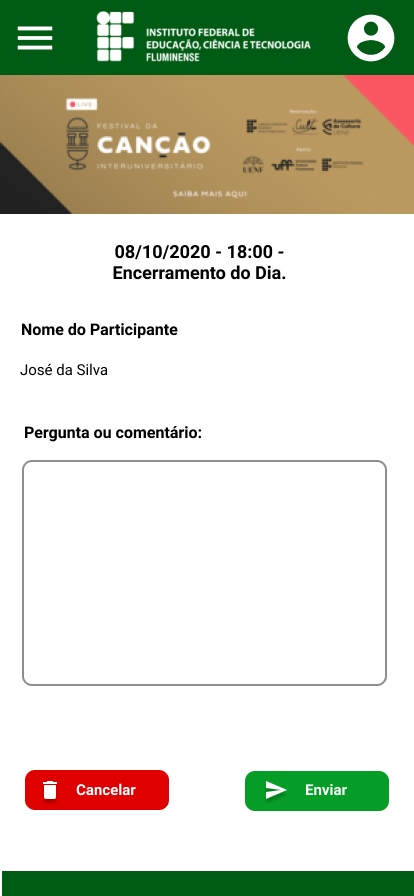
\includegraphics[scale=0.44]{figuras/Audiencia/13-EnvioComentario.jpg}
    \label{fig:audiencia13}
    \legend{Fonte: elaborado pelos autores}
\end{figure}

\section{Jornada do usuário com perfil de gestão do evento}

O fluxo inicial para os usuários com papel administrativo é o mesmo descrito na seção anterior. Ao se autenticar, o mesmo é direcionado para a tela inicial com a mesma estrutura da Figura \ref{fig:audiencia2}. Também é possível acessar os mesmos menus laterais, como na Figura \ref{fig:audiencia3} e Figura \ref{fig:audiencia4}.B, no entanto, caso o usuário tenha vinculado a ele algum evento, onde o mesmo seja organizador, palestrante ou voluntário, será apresentada uma opção adicional no menu lateral esquerdo, sendo este a opção “Meus Eventos”, como apresentado na Figura \ref{fig:gestao1}. Essa opção redireciona o usuário para a tela dos seus eventos.

\begin{figure}[H]
    \centering
    \caption{Menu lateral esquerdo com a opção "Meus Eventos"}
    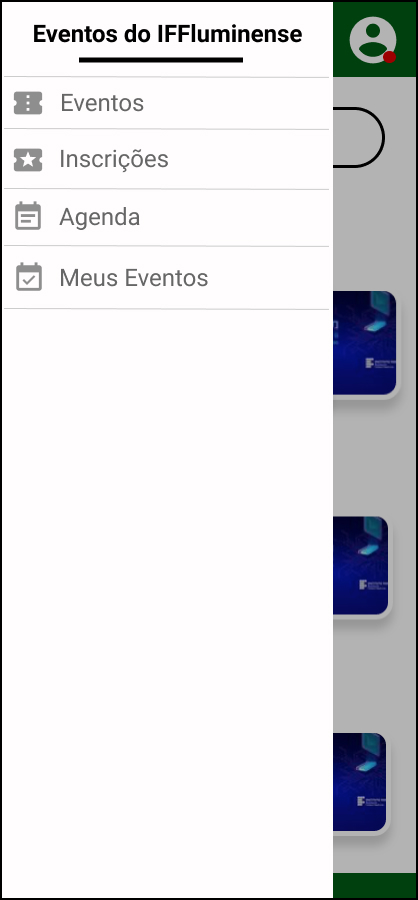
\includegraphics[scale=0.44]{figuras/Gestao/1-MenuEsquerdo.jpg}
    \label{fig:gestao1}
    \legend{Fonte: elaborado pelos autores}
\end{figure}

Na tela dos eventos do usuário (Figura \ref{fig:gestao2}.A), o mesmo tem a possibilidade de acompanhar os eventos onde ele tem algum papel administrativo, além de orientações de como solicitar a criação de um novo evento através do botão “Criar Evento”. Ao selecionar este botão, uma caixa de diálogo é apresentada indicando que o usuário poderá criar o evento através do Sistema Unificado de Administração Pública (SUAP) (Figura \ref{fig:gestao2}.B). Selecionando o botão “Ir para o SUAP” nessa caixa de diálogo, o usuário é redirecionado para o \textit{website} do SUAP.

\begin{figure}[H]
    \centering
    \caption{(A) Tela de eventos do usuário. (B) Orientação para criação de evento.}
    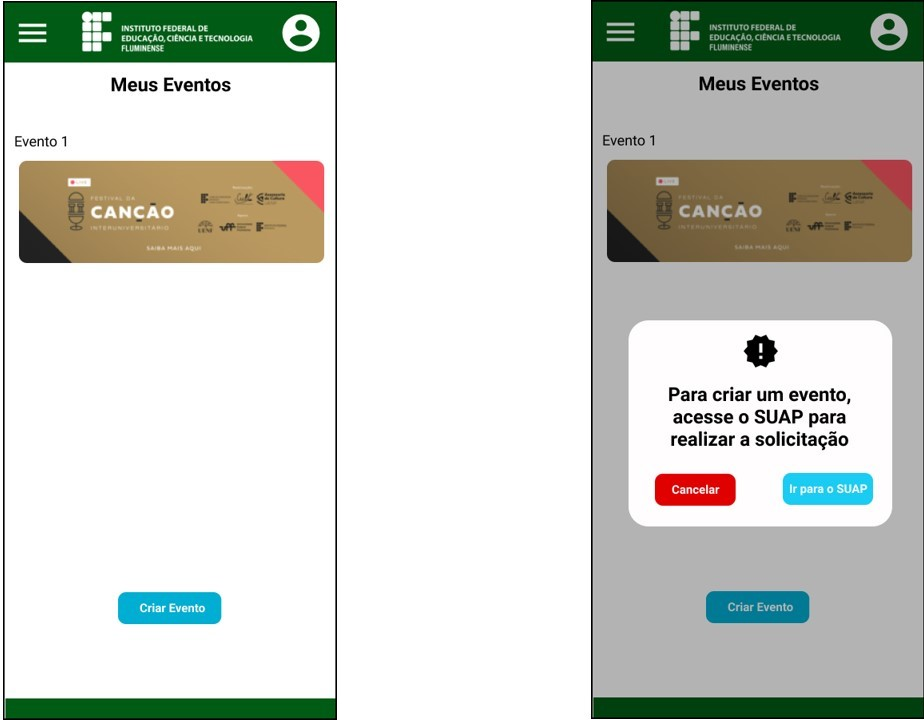
\includegraphics[scale=0.63]{figuras/Gestao/2-3.jpg}
    \label{fig:gestao2}
    \legend{Fonte: elaborado pelos autores}
\end{figure}

Na mesma tela (Figura \ref{fig:gestao2}.A), é listada os eventos em formato de cartões, onde nos cartões tem a imagem da capa do evento. Selecionando o cartão do evento, o usuário pode se deparar com duas possibilidades. Caso o evento selecionado já esteja ativado, o usuário é redirecionado para a tela de gestão do evento, a qual será detalhada posteriormente.

Entretanto, caso o evento não esteja ativado ainda, o usuário é levado para uma tela onde o mesmo poderá acompanhar o status de aprovação do evento. Isso é devido ao fato de, quando um evento é criado no SUAP, esse evento necessita de uma aprovação para estar apto para estar visível no Eventos IFF. Nessa etapa o evento pode apresentar três status em relação a essa aprovação, sendo pendente, reprovado ou aprovado. A mensagem na tela varia para cada um destes status, assim como ilustrado na Figura \ref{fig:gestao5}.

\begin{figure}[H]
    \centering
    \caption{Variação da tela de acompanhamento do status de aprovação do evento}
    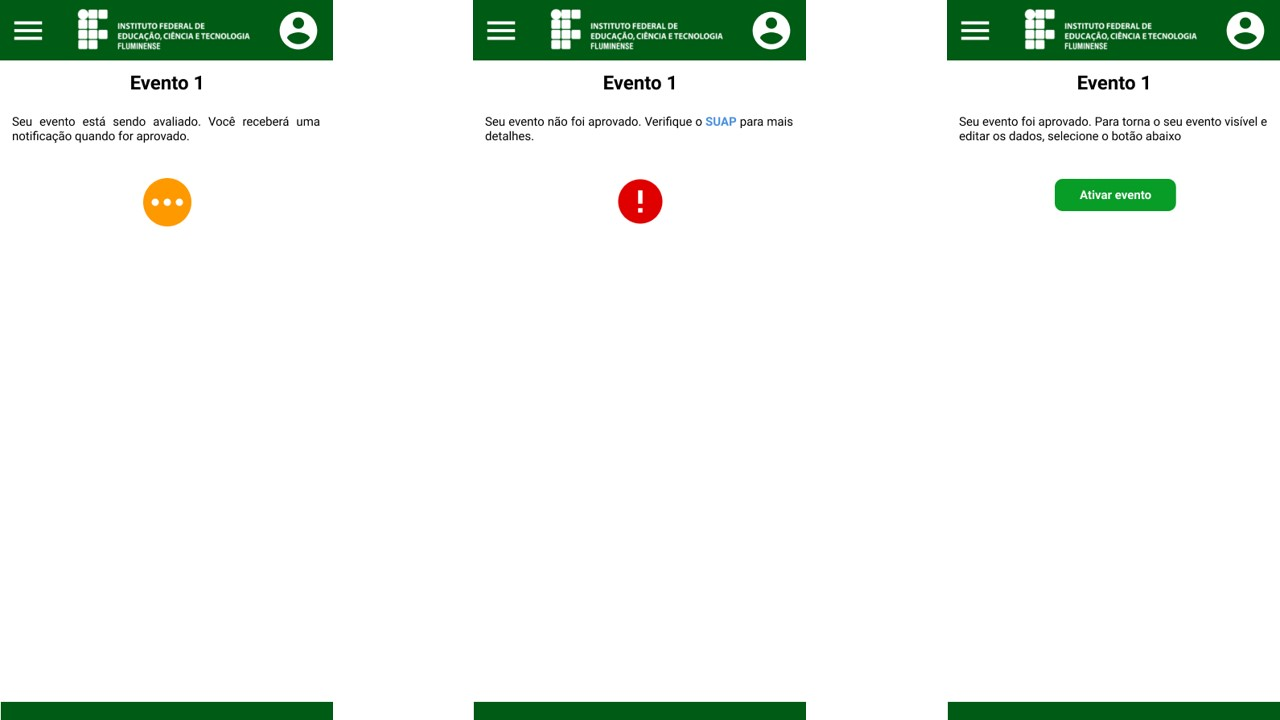
\includegraphics[scale=0.47]{figuras/Gestao/5-6-7.jpg}
    \label{fig:gestao5}
    \legend{Fonte: elaborado pelos autores}
\end{figure}

Como apresentado na Figura  \ref{fig:gestao5}, caso o evento esteja aprovado pelo SUAP e ainda não esteja ativado, o usuário poderá realizar essa ação pelo botão ‘Ativar evento’. Esta funcionalidade faz com que o evento torna-se ativo e visível no Eventos IFF.

Após o processo de ativação do evento, haverá o redirecionamento para a tela de gestão do evento (Figura \ref{fig:gestao8}). Na tela de gestão do evento, o usuário terá disponível as abas ‘Editar Dados’ e ‘Gerenciar Atividades’. Em ‘Editar Dados’, o usuário poderá editar o nome e descrição do evento, além de ter as opções para gerenciar as atividades e convidar voluntários. Também é possível conferir dados como o status do evento e o total de inscritos no momento.

\begin{figure}[H]
    \centering
    \caption{Tela de gestão do evento}
    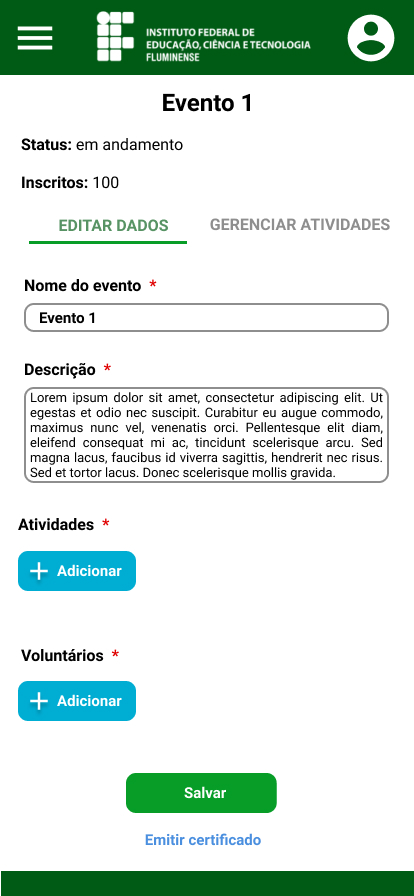
\includegraphics[scale=0.44]{figuras/Gestao/8-EditarEvento.jpg}
    \label{fig:gestao8}
    \legend{Fonte: elaborado pelos autores}
\end{figure}

Para inclusão de atividades, o usuário deverá acessar o botão ‘Adicionar’ na seção atividades, após isto o usuário será redirecionado a uma tela de criação de atividade (Figura \ref{fig:gestao9}.A). Nesta tela o usuário terá duas abas, sendo estas ‘Editar Dados’ e ‘Gerenciar Palestrante’, onde na primeira aba será feito o preenchimento de informações como nome e descrição da atividade, data, hora, local e capacidade máxima de participantes permitida na atividade. Caso o usuário queira convidar palestrantes para a atividade, o usuário deverá acessar o botão ‘Adicionar’, localizado na seção palestrantes. Após selecionar este botão, uma caixa de diálogo é aberta onde possibilita o usuário informar o \textit{e-mail} ao qual deseja enviar o convite para se tornar palestrante da atividade (Figura \ref{fig:gestao9}.B). Esse convite deve conter um texto explicativo e um \textit{link} para o usuário aceitar o convite.

\begin{figure}[H]
    \centering
    \caption{(A) Tela de criação de atividade. (B) Orientação para convidar palestrante.}
    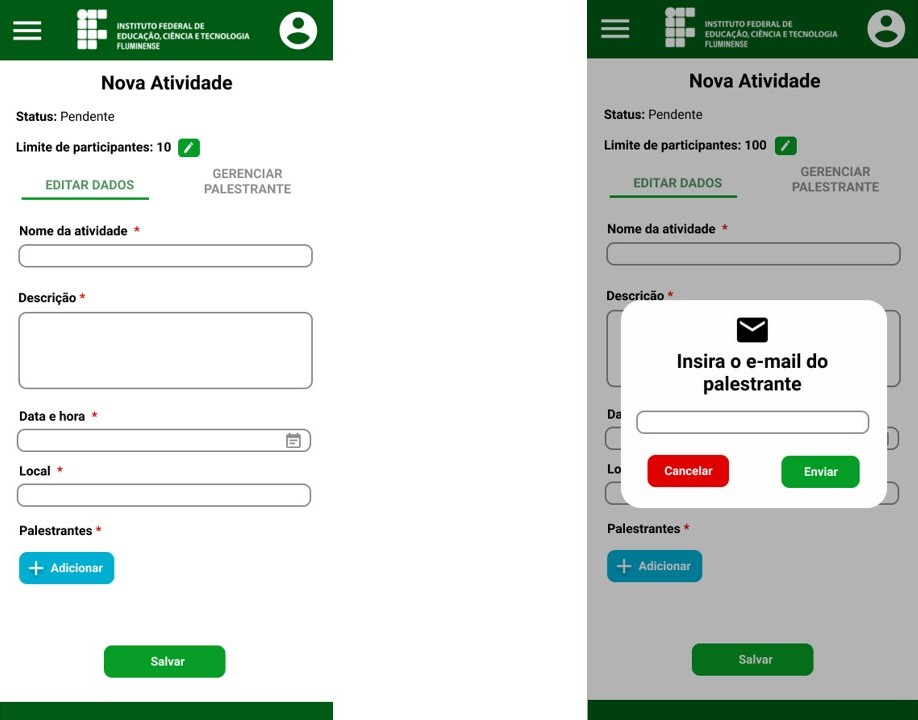
\includegraphics[scale=0.63]{figuras/Gestao/9-10.jpg}
    \label{fig:gestao9}
    \legend{Fonte: elaborado pelos autores}
\end{figure}

Na segunda aba desta mesma tela, a aba ‘Gerenciar Palestrante’, é possível realizar a gestão dos palestrantes relacionados à atividade, dando como possibilidade a exclusão dos palestrantes.

\begin{figure}[H]
    \centering
    \caption{Tela de gestão de palestrantes da atividade}
    
\includegraphics[scale=0.44]{figuras/Gestao/11-GestaoPalestrantes.jpg}
    \label{fig:gestao11}
    \legend{Fonte: elaborado pelos autores}
\end{figure}

Finalizando a criação da atividade na aba ‘Editar Dados’ citada anteriormente (Figura \ref{fig:gestao9}.A), o usuário deverá selecionar o botão "Salvar" na parte inferior da tela para disponibilizar a atividade no evento. Dessa forma ele será redirecionado à tela de gestão do evento (Figura \ref{fig:gestao8}).

Para inclusão de voluntários, o usuário deverá acessar o botão ‘Adicionar’ na seção voluntários, sendo assim levado para a tela de gestão de voluntários do evento (Figura \ref{fig:gestao12}.A). Nesta tela, o usuário terá a visibilidade de todos os usuários voluntários atualmente vinculados ao evento, possibilitando remover alguém. Para convidar um novo voluntário, basta selecionar o botão ‘Adicionar’. Essa ação irá abrir uma caixa de diálogo seguindo o mesmo padrão da ação de convite de palestrante, assim como na Figura \ref{fig:gestao12}.B. Após isso o usuário deve preencher no campo de texto exibido o \textit{e-mail} ao qual deseja enviar o convite. Este convite deve seguir o mesmo padrão do convite do palestrante citado anteriormente.

\begin{figure}[H]
    \centering
    \caption{(A) Tela de gestão de voluntários. (B) Orientação para convidar voluntário.}
    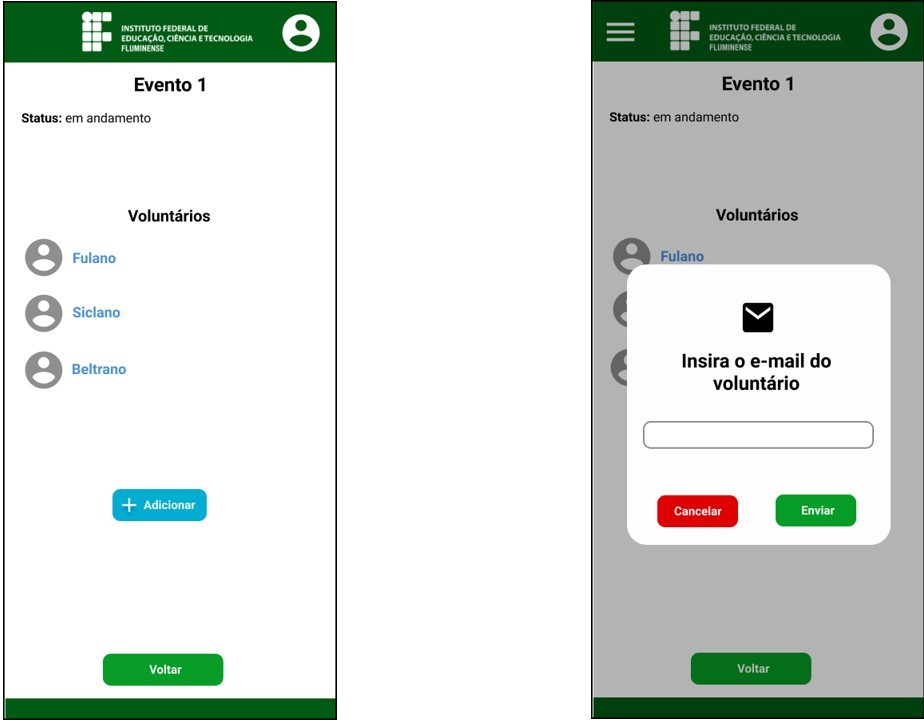
\includegraphics[scale=0.63]{figuras/Gestao/12-13.jpg}
    \label{fig:gestao12}
    \legend{Fonte: elaborado pelos autores}
\end{figure}

	
Selecionando o botão “Voltar” nesta tela (Figura \ref{fig:gestao12}.A) o usuário retorna a tela de gestão do evento, como na Figura \ref{fig:gestao8}. O usuário poderá realizar a gestão das atividades na aba ‘Gerenciar Atividades’ desta tela. Nesta aba o usuário terá a visão das atividades cadastradas no evento e poderá editá-las selecionando a atividade desejada (Figura \ref{fig:gestao14}).

\begin{figure}[H]
    \centering
    \caption{Tela de gestão das atividades do evento}
    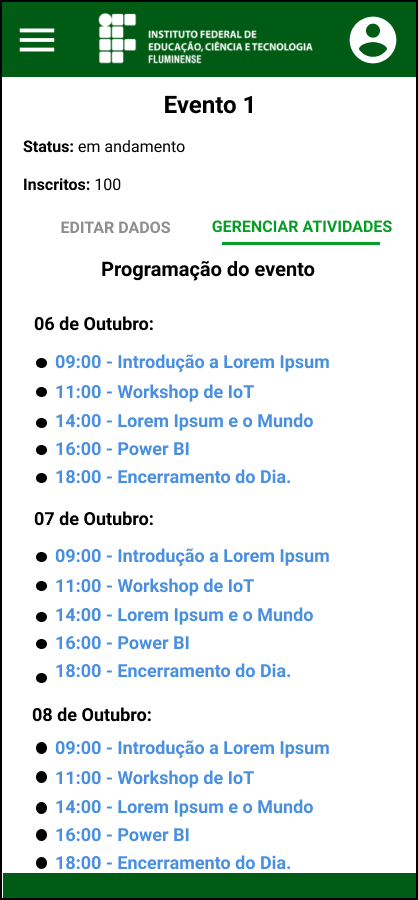
\includegraphics[scale=0.44]{figuras/Gestao/14-GerenciarAtividades.jpg}
    \label{fig:gestao14}
    \legend{Fonte: elaborado pelos autores}
\end{figure}

Ao acessar a atividade desejada o usuário terá na tela as informações a respeito da mesma, como status da atividade, capacidade máxima de participantes e data e hora do início (Figura \ref{fig:gestao15}). Além disso, o usuário poderá editar ou excluir a atividade selecionando os botões na parte superior da página. A ação de edição redireciona para a mesma tela de criação de atividade, porém com os campos de texto e demais informações já preenchidos. O usuário poderá realizar as ações de credenciamento por esta tela através de duas possibilidades. A primeira possibilidade é por meio do campo de texto, onde usuário informa a credencial do participante e seleciona o botão “Registrar presença” para concluir a ação.

\begin{figure}[H]
    \centering
    \caption{Tela da atividade selecionada}
    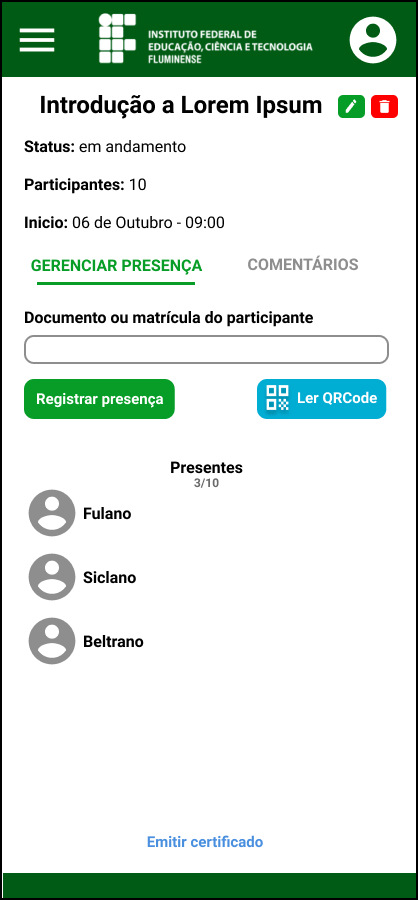
\includegraphics[scale=0.44]{figuras/Gestao/15-Atividade.jpg}
    \label{fig:gestao15}
    \legend{Fonte: elaborado pelos autores}
\end{figure}

A segunda possibilidade se dá por meio do botão “Ler \textit{QRCode}”, onde ao selecionar esse botão, o aplicativo deve abrir o leitor de \textit{QRCode} do dispositivo móvel, possibilitando realizar a leitura do \textit{QRCode} de credenciamento do participante.

Logo abaixo desta mesma tela, o usuário poderá ver a lista de participantes que já realizaram o credenciamento, assim como conseguir a informação de quantos participantes faltam realizar o credenciamento dos que confirmaram a presença anteriormente.

Para acessar os comentários do evento, o usuário deverá acessar a aba ‘Comentários’ desta tela. Nessa aba, o usuário terá a possibilidade de ler os comentários feitos pelos os participantes e realizar a gestão dos mesmos (Figura \ref{fig:gestao17}.A). Os comentários são ordenados pelo critério de avaliação citado anteriormente. Caso seja necessário excluir algum comentário, pelo o motivo, por exemplo, de o mesmo ter sido denunciado, o usuário poderá realizar essa ação deslizando o comentário para a esquerda. Isso irá habilitar o botão de exclusão do comentário para completar a ação (Figura \ref{fig:gestao17}.B).

\begin{figure}[H]
    \centering
    \caption{(A) Tela de gestão dos comentários. (B) Ação de exclusão do comentário.}
    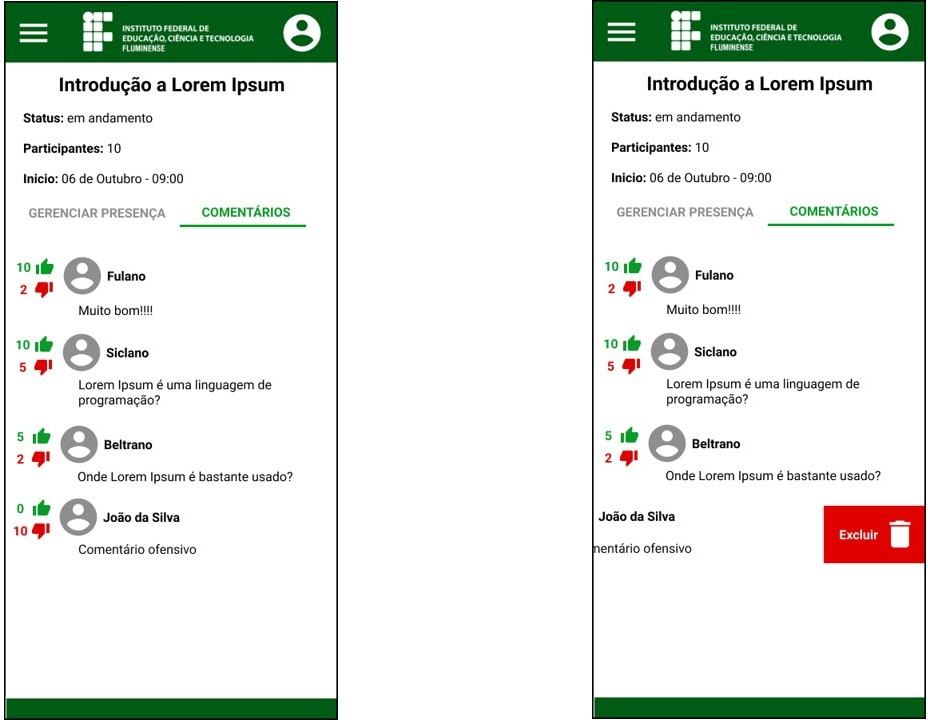
\includegraphics[scale=0.63]{figuras/Gestao/17-18.jpg}
    \label{fig:gestao17}
    \legend{Fonte: elaborado pelos autores}
\end{figure}

Finalizando, é importante destacar que essa jornada da gestão de evento descrita por essa seção pode ter como três tipos de usuário vinculados por evento, sendo estes organizador, palestrante e voluntário. O usuário organizador consegue executar todas as funcionalidades descritas nesta jornada, sendo o usuário criador do evento já atribuído automaticamente como organizador. 

O usuário voluntário se limita apenas às ações de realizar credenciamento em atividade, editar atividade, denunciar comentários e excluir comentários. O usuário palestrante pode apenas executar ações na atividade a qual está vinculado. Essas ações são:  realizar credenciamento em atividade, denunciar comentários e excluir comentários.
